%! TeX program = lualatex
\documentclass[../main.tex]{subfiles}

\ifcsname preamble@file\endcsname
  \externaldocument[main-]{../../build/main}
  \setcounter{page}{\getpagerefnumber{main-week9}}
\fi

\begin{document} \makelectureweek{9}

\section{Extreme Values}
\begin{mdframed}[style=withref]
  Let \(c\) be a number in the domain \(D\) of a function \(f\). Then \(f(c)\) is called the
  \begin{itemize}
    \item \emph{absolute (or global) maximum} value of \(f\) if \(f(c) \hspace{2em} f(x)\) for all \(x \in D\).

    \item \emph{absolute (or global) minimum} value of \(f\) if \(f(c) \hspace{2em} f(x)\) for all \(x \in D\).

    \item \emph{local maximum} value of \(f\) if \(f(c) \hspace{2em} f(x)\) when \(x\) is near \(c\).

    \item \emph{local minimum} value of \(f\) if \(f(c) \hspace{2em} f(x)\) when \(x\) is near \(c\).
  \end{itemize}
  \textbook{\stewart{280}{\fbox{1} Defintion \textcolor{black}{and} \fbox{2} Defintion}}
\end{mdframed}
Maximum and minimum values are called \emph{extreme} values.

\begin{center}
  \begin{tikzpicture}
    \draw[dotted, thin] (0,0) grid[step=0.5] (5,4);
    \draw[->] (0,0) -- (0,4);
    \draw[->] (0,0) -- (5,0);
    \foreach \n in {1,2,3,4,4} {
      \draw (0.04,\n) -- (-0.04,\n) node[left] {\footnotesize \(\n\)};
      \draw (\n,0.04) -- (\n,-0.04) node[below] {\footnotesize \(\n\)};
    }
  \end{tikzpicture}
  \hfill
  \begin{tikzpicture}
    \draw[dotted, thin] (0,0) grid[step=0.5] (5,4);
    \draw[->] (0,0) -- (0,4);
    \draw[->] (0,0) -- (5,0);
    \foreach \n in {1,2,3,4,4} {
      \draw (0.04,\n) -- (-0.04,\n) node[left] {\footnotesize \(\n\)};
      \draw (\n,0.04) -- (\n,-0.04) node[below] {\footnotesize \(\n\)};
    }
  \end{tikzpicture}
  \hfill
  \begin{tikzpicture}
    \draw[dotted, thin] (0,0) grid[step=0.5] (5,4);
    \draw[->] (0,0) -- (0,4);
    \draw[->] (0,0) -- (5,0);
    \foreach \n in {1,2,3,4} {
      \draw (0.04,\n) -- (-0.04,\n) node[left] {\footnotesize \(\n\)};
      \draw (\n,0.04) -- (\n,-0.04) node[below] {\footnotesize \(\n\)};
    }
  \end{tikzpicture}
\end{center}
\vfill

``Near \(c\)'' means ``on an \emph{open} interval containing \(c\).''  That means
\begin{enumerate}
  \item \emph{local} extreme values \emph{cannot} occur at endpoints of a \emph{closed} interval. 
  \item \emph{global} extreme values \emph{can} occur at endpoints of a \emph{closed} interval.
\end{enumerate}
\begin{center}
  \begin{tikzpicture}
    \draw[dotted, thin] (0,0) grid[step=0.5] (5,4);
    \draw[->] (0,0) -- (0,4);
    \draw[->] (0,0) -- (5,0);
    \foreach \n in {1,2,3,4} {
      \draw (0.04,\n) -- (-0.04,\n) node[left] {\footnotesize \(\n\)};
      \draw (\n,0.04) -- (\n,-0.04) node[below] {\footnotesize \(\n\)};
    }
  \end{tikzpicture}
  \hfill
  \begin{tikzpicture}
    \draw[dotted, thin] (0,0) grid[step=0.5] (5,4);
    \draw[->] (0,0) -- (0,4);
    \draw[->] (0,0) -- (5,0);
    \foreach \n in {1,2,3,4} {
      \draw (0.04,\n) -- (-0.04,\n) node[left] {\footnotesize \(\n\)};
      \draw (\n,0.04) -- (\n,-0.04) node[below] {\footnotesize \(\n\)};
    }
  \end{tikzpicture}
  \hfill
  \begin{tikzpicture}
    \draw[dotted, thin] (0,0) grid[step=0.5] (5,4);
    \draw[->] (0,0) -- (0,4);
    \draw[->] (0,0) -- (5,0);
    \foreach \n in {1,2,3,4} {
      \draw (0.04,\n) -- (-0.04,\n) node[left] {\footnotesize \(\n\)};
      \draw (\n,0.04) -- (\n,-0.04) node[below] {\footnotesize \(\n\)};
    }
  \end{tikzpicture}
\end{center}
\clearpage
 
\begin{mdframed}[style=withref]
  \textbf{The Extreme Value Theorem}. If \(f\) is \emph{continuous} on a \emph{closed} interval \([a,b]\), then \(f\) attains an absolute maximum value \(f(c)\) \emph{and} an absolute minimum value \(f(d)\) at some numbers \(c\) and \(d\) in \([a,b]\).

  \textbook{\stewart{281}{\fbox{3}}}
\end{mdframed}

The two conditions in the hypothesis (the ``if \ldots{}'' part) are very important. Let's see what can go wrong if one of these conditions is missing.
\medskip

\begin{enumerate}
  \item Is the following statement true? 

    \begin{minipage}{.4\textwidth}
      \begin{tikzpicture}
        \draw[dotted, thin] (0,0) grid[step=0.5] (5,4);
        \draw[->] (0,0) -- (0,4);
        \draw[->] (0,0) -- (5,0);
        \foreach \n in {1,2,3,4} {
          \draw (0.04,\n) -- (-0.04,\n) node[left] {\footnotesize \(\n\)};
          \draw (\n,0.04) -- (\n,-0.04) node[below] {\footnotesize \(\n\)};
        }
      \end{tikzpicture}
    \end{minipage}
    \begin{minipage}{.55\textwidth}
      \vspace{-2.5cm}
      \textit{If \(f\) is defined on a \emph{closed} interval \([a,b]\), then \(f\) attains an absolute maximum value \(f(c)\) \emph{and} an absolute minimum value \(f(d)\) at some numbers \(c\) and \(d\) in \([a,b]\).}
    \end{minipage}

    \vfill

  \item Is the following statement true? 

    \begin{minipage}{.4\textwidth}
      \begin{tikzpicture}
        \draw[dotted, thin] (0,0) grid[step=0.5] (5,4);
        \draw[->] (0,0) -- (0,4);
        \draw[->] (0,0) -- (5,0);
        \foreach \n in {1,2,3,4} {
          \draw (0.04,\n) -- (-0.04,\n) node[left] {\footnotesize \(\n\)};
          \draw (\n,0.04) -- (\n,-0.04) node[below] {\footnotesize \(\n\)};
        }
      \end{tikzpicture}
    \end{minipage}
    \begin{minipage}{.55\textwidth}
      \vspace{-2cm}
      \textit{If \(f\) is continuous on an open interval \((a,b)\), then \(f\) attains an absolute maximum value \(f(c)\) \emph{and} an absolute minimum value \(f(d)\) at some numbers \(c\) and \(d\) in \((a,b)\).}
    \end{minipage}

    \vfill

  \item Is the following statement true? 


    \begin{minipage}{.4\textwidth}
      \begin{tikzpicture}
        \draw[dotted, thin] (0,0) grid[step=0.5] (5,4);
        \draw[->] (0,0) -- (0,4);
        \draw[->] (0,0) -- (5,0);
        \foreach \n in {1,2,3,4} {
          \draw (0.04,\n) -- (-0.04,\n) node[left] {\footnotesize \(\n\)};
          \draw (\n,0.04) -- (\n,-0.04) node[below] {\footnotesize \(\n\)};
        }
      \end{tikzpicture}
    \end{minipage}
    \begin{minipage}{.55\textwidth}
      \vspace{-2cm}
      \textit{If \(f\) is continuous on a half-open interval \(I\), then \(f\) attains an absolute maximum value \(f(c)\) \emph{and} an absolute minimum value \(f(d)\) at some numbers \(c\) and \(d\) in \(I\).}
    \end{minipage}
\end{enumerate}
\clearpage

\begin{mdframed}[style=withref]
  \textbf{Theorem} (Fermat). If a function \(f\) has a local maximum or minimum at \(c\), and if \(f'(c)\) exists, then \(f'(c) = 0\).

  \textbook{\stewart{282}{\fbox{4}}}
\end{mdframed}
\bigskip

\begin{mdframed}[style=withref]
  A \textbf{critical number} of a function \(f\) is a number \(c\) in the \emph{domain} of \(f\) such that 
  \[
    f'(c) = 0 \quad\text{or}\quad f'(c) \text{ does not exist}.
  \]

  \textbook{\stewart{282}{\fbox{6} Definition}}
\end{mdframed}
\faExclamationTriangle{} Critical numbers only have the \emph{potential} to be local extreme values. The following examples demonstrate that \emph{not} all critical numbers correspond to local extreme values. 


% If \(c\) is a critical number, we still don't know whether \(f(c)\) is a local minimum or maximum.
\begin{center}
\begin{tikzpicture}
  \draw[dotted, thin] (0,0) grid[step=0.5] (5,4);
  \draw[->] (0,0) -- (0,4);
  \draw[->] (0,0) -- (5,0);
  \foreach \n in {1,2,3,4} {
    \draw (0.04,\n) -- (-0.04,\n) node[left] {\footnotesize \(\n\)};
    \draw (\n,0.04) -- (\n,-0.04) node[below] {\footnotesize \(\n\)};
  }
\end{tikzpicture}
\hspace{1in}
\begin{tikzpicture}
  \draw[dotted, thin] (0,0) grid[step=0.5] (5,4);
  \draw[->] (0,0) -- (0,4);
  \draw[->] (0,0) -- (5,0);
  \foreach \n in {1,2,3,4} {
    \draw (0.04,\n) -- (-0.04,\n) node[left] {\footnotesize \(\n\)};
    \draw (\n,0.04) -- (\n,-0.04) node[below] {\footnotesize \(\n\)};
  }
\end{tikzpicture}
\end{center}
\medskip

\faExclamationTriangle{} Even if a critical number is local extreme value, we still do not know whether it is a local maximum or a local minimum.
\vspace{1in}

\begin{example} \label{ref:ex-critical-numbers}
  Find critical numbers of \(f(x) = x^{5}\) on \([-1,1]\). Which critical numbers(s) do not correspond to local extreme value(s)?
\end{example}
\vfill
\clearpage

\begin{mdframed}[style=withref]
  To find the absolute maximum and minimum value of a \emph{continuous} functionon a \emph{closed} interval \([a,b]\).
  \begin{enumerate}
  \item Find the values of \(f\) at the critical numbers of \(f\) in \((a,b)\).
  \item Find the \(f(a)\) and \(f(b)\).
  \item The largest values from Steps~1~and~2 is the absolute maximum; the smallest value is the absolute minimum.
  \end{enumerate}

  \textbook{\stewart{284}{The Closed Interval Method}}
\end{mdframed}

\begin{example}
  Find the absolute maximum and minimum values of \(f(x) = \frac{1}{3} x^{3} - \frac{3}{2} x^{2} + 2x\) on \([0,5/2]\).
\end{example}
\vfill
\clearpage
%
% \begin{example}
%   Find the absolute extreme values of the function \(f(x) = x - 5 \sqrt[5]{x}\) on \([-1,2]\).
% \end{example}
% \clearpage

\section{\(f'\) and Intervals of Increasing and Decreasing}
\begin{center}
  \includegraphics[scale=0.8]{../standalones/build/plot_increasing_decreasing}
  \hfill
  \includegraphics[scale=0.8]{../standalones/build/plot_increasing_decreasing_only_derivative}
  \hfill
  \includegraphics[scale=0.8]{../standalones/build/plot_increasing_decreasing_with_derivative}
\end{center}
\vspace{1in}

\begin{mdframed}[style=withref]
  \textbf{Theorem} (Increasing/Decreasing Test). 
  \begin{enumerate}[label=(\alph*)]
    \item If \(f'(x) \hspace{2em} 0\) for every \(x\) in \(I\), then \(f(x)\) is increasing on \(I\).
    \item If \(f'(x) \hspace{2em} 0\) for every \(x\) in \(I\), then \(f(x)\) is decreasing on \(I\).
  \end{enumerate}

  \textbook{\stewart{297}{Increasing/Decreasing Test}}
\end{mdframed}

\faComments{} If \(f'(c) = 0\) at some number \(c\), then is \(f(x)\) is increasing or decreasing (or neither) at \(c\)?
\vspace{1cm}

\begin{example}
  Consider the graph of \(f'(x)\) below. Label the interval on which \(f(x)\) is increasing. 

  \begin{minipage}{0.4\textwidth}
    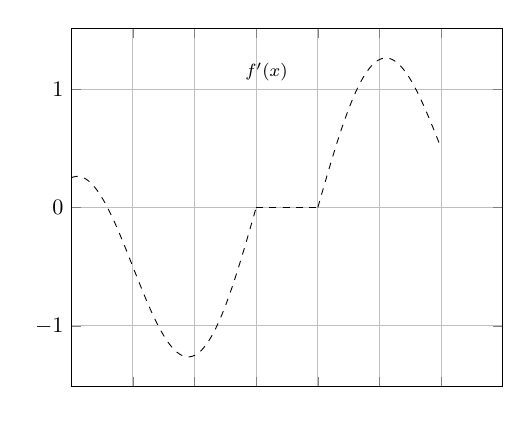
\begin{tikzpicture}[scale=0.8]
      \begin{axis}[
        % ymin=0, ymax=1,  
        xmin=-3*pi/2, xmax=2*pi,
        xtick={-3*pi/2, -pi, -pi/2, 0, pi/2, pi, 3*pi/2},
        xticklabels={,,},
        smooth,
        samples=100,
        no markers,
        grid=both,
        ]
        \addplot[dashed, black, domain=-3*pi/2:0] {sin(deg(x)) + x/2/pi};
        \addplot[dashed, black, domain=0:pi/2] {0};
        \addplot[dashed, black, domain=pi/2:3*pi/2] {sin(deg(x-pi/2)) + (x-pi/2)/2/pi};
        \node[above left] at (axis cs:1,1) {\footnotesize \(f'(x)\)};
      \end{axis}
    \end{tikzpicture}
  \end{minipage}
  \begin{minipage}{0.59\textwidth}
    \vspace{-1in}
    \footnotesize
    You might find this trick useful: Translate the quesion into an everyday life question.
    \medskip

    Pretent \(f'\) is the velocity function of a car. Then \(f\) becomes the displacement function of a car. 
  \end{minipage}

\end{example}

% \faComments{} Can we use the I/D Test useful to find local extreme values?
% \vspace{1cm}

\clearpage

\begin{example} \label{ex:first-derivative}
  Determine intervals of increase or decrease of \(f(x) = 2x^{3} - 9x^{2} + 12x\).
\end{example}
\clearpage

\begin{mdframed}[style=withref]
  \textbf{Theorem} (The First Derivative Test). Suppose that \(c\) is a critical number of a continuous function \(f\). 
  \begin{enumerate}
    \item  If \(f'\) \emph{changes} from positive to negative, then \(f\) has a local maximum at \(c\).
    \item  If \(f'\) \emph{changes} from negative to positive, then \(f\) has a local minimum at \(c\).
    \item  If \(f'\) is positive to the left and right of \(c\), or negative to the left and right of \(c\), then \(f\) has \emph{no} local maximum or minimum at \(c\).
  \end{enumerate}

  \textbook{\stewart{298}{The First Derivative Test}}
\end{mdframed}
The First Derivative Test simply says the following in the language of the first derivative. 
\begin{enumerate}
  \item If \(f\) changes from {increasing} to {decreasing} at \(c\), then \(f\) has a local maximum at \(c\).
  \item If \(f\) changes from {decreasing} to {increasing} at \(c\), then \(f\) has a local minimum at \(c\).
  \item If \(f\) is {increasing} to the left and right of \(c\), or {decreasing} to the left and right of \(c\), then \(f\) has no local maximum or minimum at \(c\).
\end{enumerate}
\bigskip

\begin{example}
  Determine local minimum(s) and local maximum(s) of \(f(x) = 2x^{3} - 9x^{2} + 12x\) from Example~\ref{ex:first-derivative}.
\end{example}
\clearpage

\section{\(f''\) and Concavity}

\begin{center}
  \includegraphics[scale=0.8]{../standalones/build/plot_concave_upward}
  \hfill
  \includegraphics[scale=0.8]{../standalones/build/plot_concave_downward}
  \hfill
  \includegraphics[scale=0.8]{../standalones/build/plot_concave_updown}
\end{center}
\bigskip

\begin{mdframed}[style=withref]
  \begin{itemize}
    \item If the graph of \(f\) lies {above} all of its tangent lines on an interval \(I\), then \(f\) is called \emph{concave upward} on \(I\). 
    \item If the graph of \(f\) lies {below} all of its tangent lines on an interval \(I\), then \(f\) is called \emph{concave downward} on \(I\).
  \end{itemize}

  \textbook{\stewart{300}{Definition}}
\end{mdframed}

A point \(P\) \emph{on the curve} \(y = f(x)\) is called an \emph{inflection point} if \(f\) is continuous there and the curve changes from concave upward to concave downward \emph{or} from concave downward to concave upward at \(P\).

\vspace{1in}

\begin{center}
  \includegraphics[scale=0.8]{../standalones/build/plot_concavity}
  \hfill
  \includegraphics[scale=0.8]{../standalones/build/plot_concavity_only_derivative}
  \hfill
  \includegraphics[scale=0.8]{../standalones/build/plot_concavity_with_derivative}
\end{center}

\begin{mdframed}[style=withref]
  \textbf{Theorem} (Concavity Test). 
  \begin{enumerate}[label=(\alph*)]
    \item If \(f''(x) \hspace{2em} 0\) on an interval \(I\), then the graph of \(f\) is \emph{concave upward} on \(I\).
    \item If \(f''(x) \hspace{2em} 0\) on an interval \(I\), then the graph of \(f\) is \emph{concave downward} on \(I\).
  \end{enumerate}

  \textbook{\stewart{300}{Concavity Test}}
\end{mdframed}

\clearpage

\begin{example} \label{ex:concavity}
  Find inflection points of \(f(x) = x^{4} - 4x^{3}\) and determine intervals on which \(f(x)\) are concave upward or concave downward. 
\end{example}
\vfill

\begin{mdframed}[style=withref]
  \textbf{Theorem}. Suppose \(f''\) is continuous near \(c\). 
  \begin{enumerate}[label=(\alph*)]
  \item If \(f'(c) = 0\) and \(f''(c) > 0\), then \(f\) has a local minimum at \(c\).
  \item If \(f'(c) = 0\) and \(f''(c) < 0\), then \(f\) has a local maximum at \(c\).
  \item[\faExclamationTriangle{}] If \(f'(c) = 0\) but \(f''(c) = 0\) or \(f''(c)\) does not exists, then the Second Derivative Test is inconclusive and we need to explore other methods to find local extreme values.
  \end{enumerate}

  \textbook{\stewart{302}{The Second Derivative Test}}
\end{mdframed}

\begin{example}
  Find local extreme values of the function \(f(x) = x^{4} - 4x^{3}\) from Example~\ref{ex:concavity}.
\end{example}
\vfill
\clearpage

Make up the graph of a function \(f\) of time (in the graphing paper below) with 
at least \(3\) local extreme values,
at least \(1\) global extreme value, and
at least \(1\) critical number that does not correspond to an extreme value.

Make up a story about your graph by coming up with events whenever there is an extreme value.
\bigskip
\begin{center}
  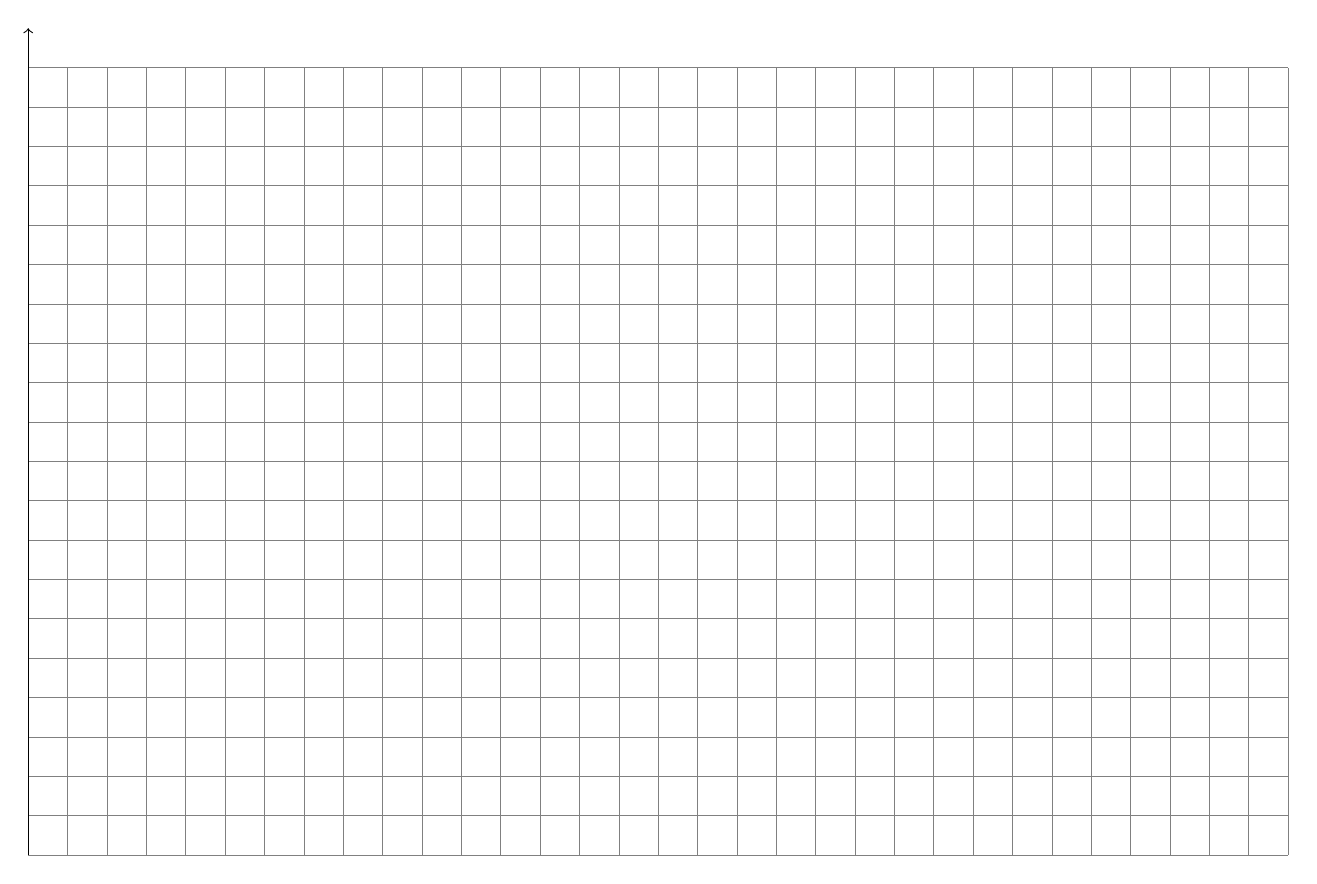
\begin{tikzpicture}
    \draw[very thin, gray] (0,0) grid[step=0.5] (16,10);
    \draw[->] (0,0) -- (0,10.5);
  \end{tikzpicture}
\end{center}

Do intervals of increase/decrease on the graph correspond something in your story?
\vfill

Do intervals of concave upwards/downward on the graph correspond to something in your story?
\vfill

Do inflection points correspond to any events in your story?
\vfill

\clearpage

\section{The Mean Value Theorem}

\faComment{} If a car travels \(200\) km in \(2\) hours, does the car have to reach \(100\) km/h at least once during this time? 

\begin{center}
  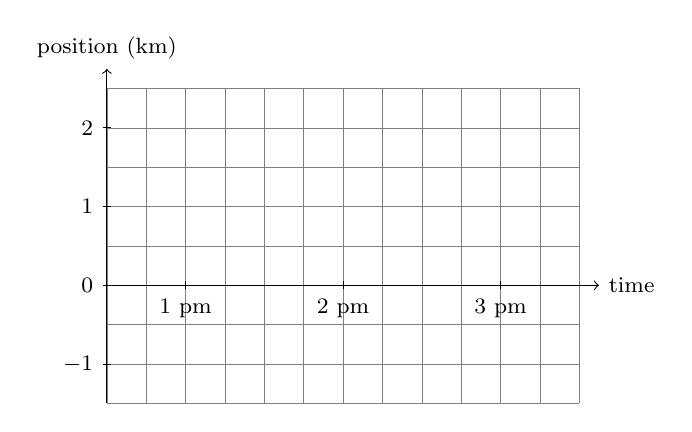
\begin{tikzpicture}
    \draw[very thin, gray] (0,0) grid[step=0.5] (6,4);
    \draw[->] (0,1.5) -- (6.25,1.5) node[right] {\footnotesize time};
    \draw[->] (0,0) -- (0,4.25) node[above] {\footnotesize position (km)};
    \foreach \n in {1,2,3} {
      \draw ({\n*2-1}, {1.5+0.05}) -- ({\n*2-1}, {1.5-0.05}) node[below] {\footnotesize \(\n\) pm};
    }
    \foreach \n in {-1,0,1,2} {
      \draw (0.05, {\n+1.5}) -- (-0.05, {\n+1.5}) node[left] {\footnotesize \(\n\)};
    }
  \end{tikzpicture}
  \quad{}
  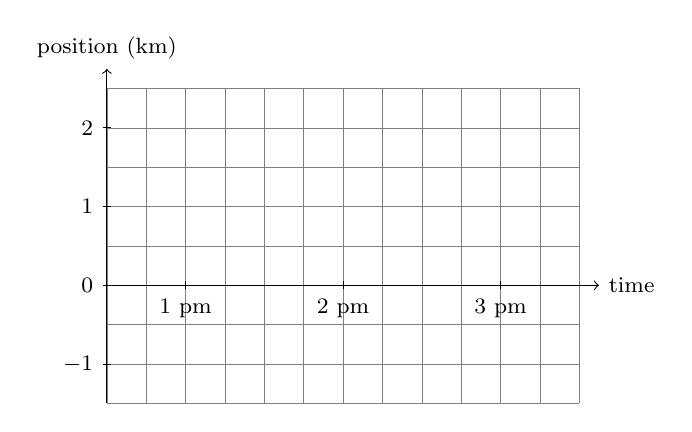
\begin{tikzpicture}
    \draw[very thin, gray] (0,0) grid[step=0.5] (6,4);
    \draw[->] (0,1.5) -- (6.25,1.5) node[right] {\footnotesize time};
    \draw[->] (0,0) -- (0,4.25) node[above] {\footnotesize position (km)};
    \foreach \n in {1,2,3} {
      \draw ({\n*2-1}, {1.5+0.05}) -- ({\n*2-1}, {1.5-0.05}) node[below] {\footnotesize \(\n\) pm};
    }
    \foreach \n in {-1,0,1,2} {
      \draw (0.05, {\n+1.5}) -- (-0.05, {\n+1.5}) node[left] {\footnotesize \(\n\)};
    }
  \end{tikzpicture}
\end{center}

\begin{mdframed}[style=withref]
  \textbf{Theorem}. If \hlmain{a function \(f\) is \emph{continuous} on a closed interval \([a,b]\) and \emph{differentiable} on the open interval \((a,b)\)}, then \textcolor{blue}{there exists a number \(c\) in \((a,b)\) such that }
  \begin{equation} \label{eq:mvt}
    f'(c) = \frac{f(b) - f(a)}{b - a}.
  \end{equation}

  \textbook{\stewart{291}{The Mean Value Theorem}}
\end{mdframed}

\begin{mdframed}[style=withref]
  \textbf{Theorem}. If \hlmain{a function \(g\) is continuous on a closed interval \([a,b]\) and \emph{differentiable} on the open interval \((a,b)\)} {\hlattn{\emph{and} \(g(a) = g(b)\)}}, then there exists a number \(c\) in \((a,b)\) such that
  \begin{equation} \label{eq:rolle}
    {g'(c) = 0.}
  \end{equation}

  \textbook{\stewart{290}{Rolle's Theorem}}
\end{mdframed}
\bigskip

Rolle's Theorem appears to be a special case of MVT.  However, Rolle's Theorem and MVT are logically equivalent, meaning MVT implies Rolle's Theorem \emph{and} Rolle's Theorem implies MVT. 

On the next page, we demonstrate how to prove that Rolle's Theorem \emph{implies} Rolle's Theorem. 
\begin{enumerate}
  \item We begin the proof by assuming a function \(f\) satisfies the \hlmain{hypothesis} of MVT.
  \item We are \emph{not} allowed to apply the MVT anywhere in the proof.
  \item We are allowed to apply Rolle's theorem in the proof.
  \item We end the proof by showing the \textcolor{blue}{conclusion} of MVT is true.
\end{enumerate}

\clearpage
Proof (Rolle's Theorem implies MVT). 

Visualization of the proof idea: \url{https://www.geogebra.org/calculator/bcsszgna}.

\clearpage
The Mean Value Theorem has theoretical importance. The following (rather intuitive) theorem and its collorary allow us to compare function by calculating their derivatives. 
\bigskip

\begin{FlushRight}
\footnotesize{\textbook{\stewart{294}{\fbox{5} Theorem}}}
\end{FlushRight}
\textbf{Theorem}. If \(f'(x) = 0\) for all \(x\) in an interval \((a,b)\), then \(f\) is constant on \((a,b)\).
\vfill


\begin{FlushRight}
\footnotesize{\textbook{\stewart{294}{\fbox{6} Collorary}}}
\end{FlushRight}
\textbf{Collorary}. If \(f'(x) = g'(x)\) for all \(x\) in an interval \((a,b)\), then \(f-g\) is a constant on \((a,b)\). 
\vspace{2in}
\clearpage

\begin{example}
  Show the function \(f(x) = x^{3} - 3x + 2\) on the interval \([-2,2]\) satisfies the hypothesis of MVT. Find all number \(c\) that satisfy the conclusion of MVT.
\end{example}

\end{document}
